\subsection{Validation} \label{s:N_II:validation}

To test our hypothesis apart from the usual graphs used to analyse the networks (see below the list) there was some biological interpretation performed. This included running GO analysis and understanding which communities contributed to the subtypes.


% Network validation 
\subsubsection{Non-tumour vs Tumour Network} 

To study the differences between the non-tumour and tumour networks the previously used graph metrics (degree, pageRank, closeness, betwenees and IVI)\footnote{Reminder: the degree - node's number of connections; pageRank - node's centrality; closeness - how close the nodes are; betwenees - nodes between; IVI - a combination of network metrics} are shown in \cref{fig:N_II:net_metrics_comp}. There are four networks compared, the standard (red) and reward (green) for tumour derived, and the correspondent for non-tumour (mustard - standard and blue - reward).

% Degreee & PageRank
In the pageRank and degree metrics, the non-tumour networks seems to be elongated on the Y-axis, denoting a a high variance between the nodes. This is further enforced by the reward modifier, suggesting that there is a subset of nodes that have a high number of connections and are central to the network. Compared to the non-tumour, the TCGA derived graphs have nodes that are more similar in their centrality and the number of connections. The tumour networks having similar values for centrality and degree. 

% Closeness & betweneess
A distinct feature of the tumour networks is that there the there are a subset of genes that are close together given by the closeness plot. The reward non-tumour network has the nodes closer compared with the standard, indicating the reward modifier 'brings' the node closer. Another distinct feature of the tumour networks is that the two networks genes with high betwenees values. Again, the reward modifier amplifies this compared to the standard (this is not very clear).

% IVI
The IVI distribution for the two tumour networks are largely similar, but there is a noticeable between the non-tumour standard and reward graphs. It can be seen that the when the weight modifier is applied, the distribution is sparser, havig a subset of genes that have higher values.

Overall the metrics comparisons shows that the non-tumour network react stronger to the reward modifiers and that there is a subset of genes that are more central and have a large number of connections.

\begin{figure}[H]    
    \centering
    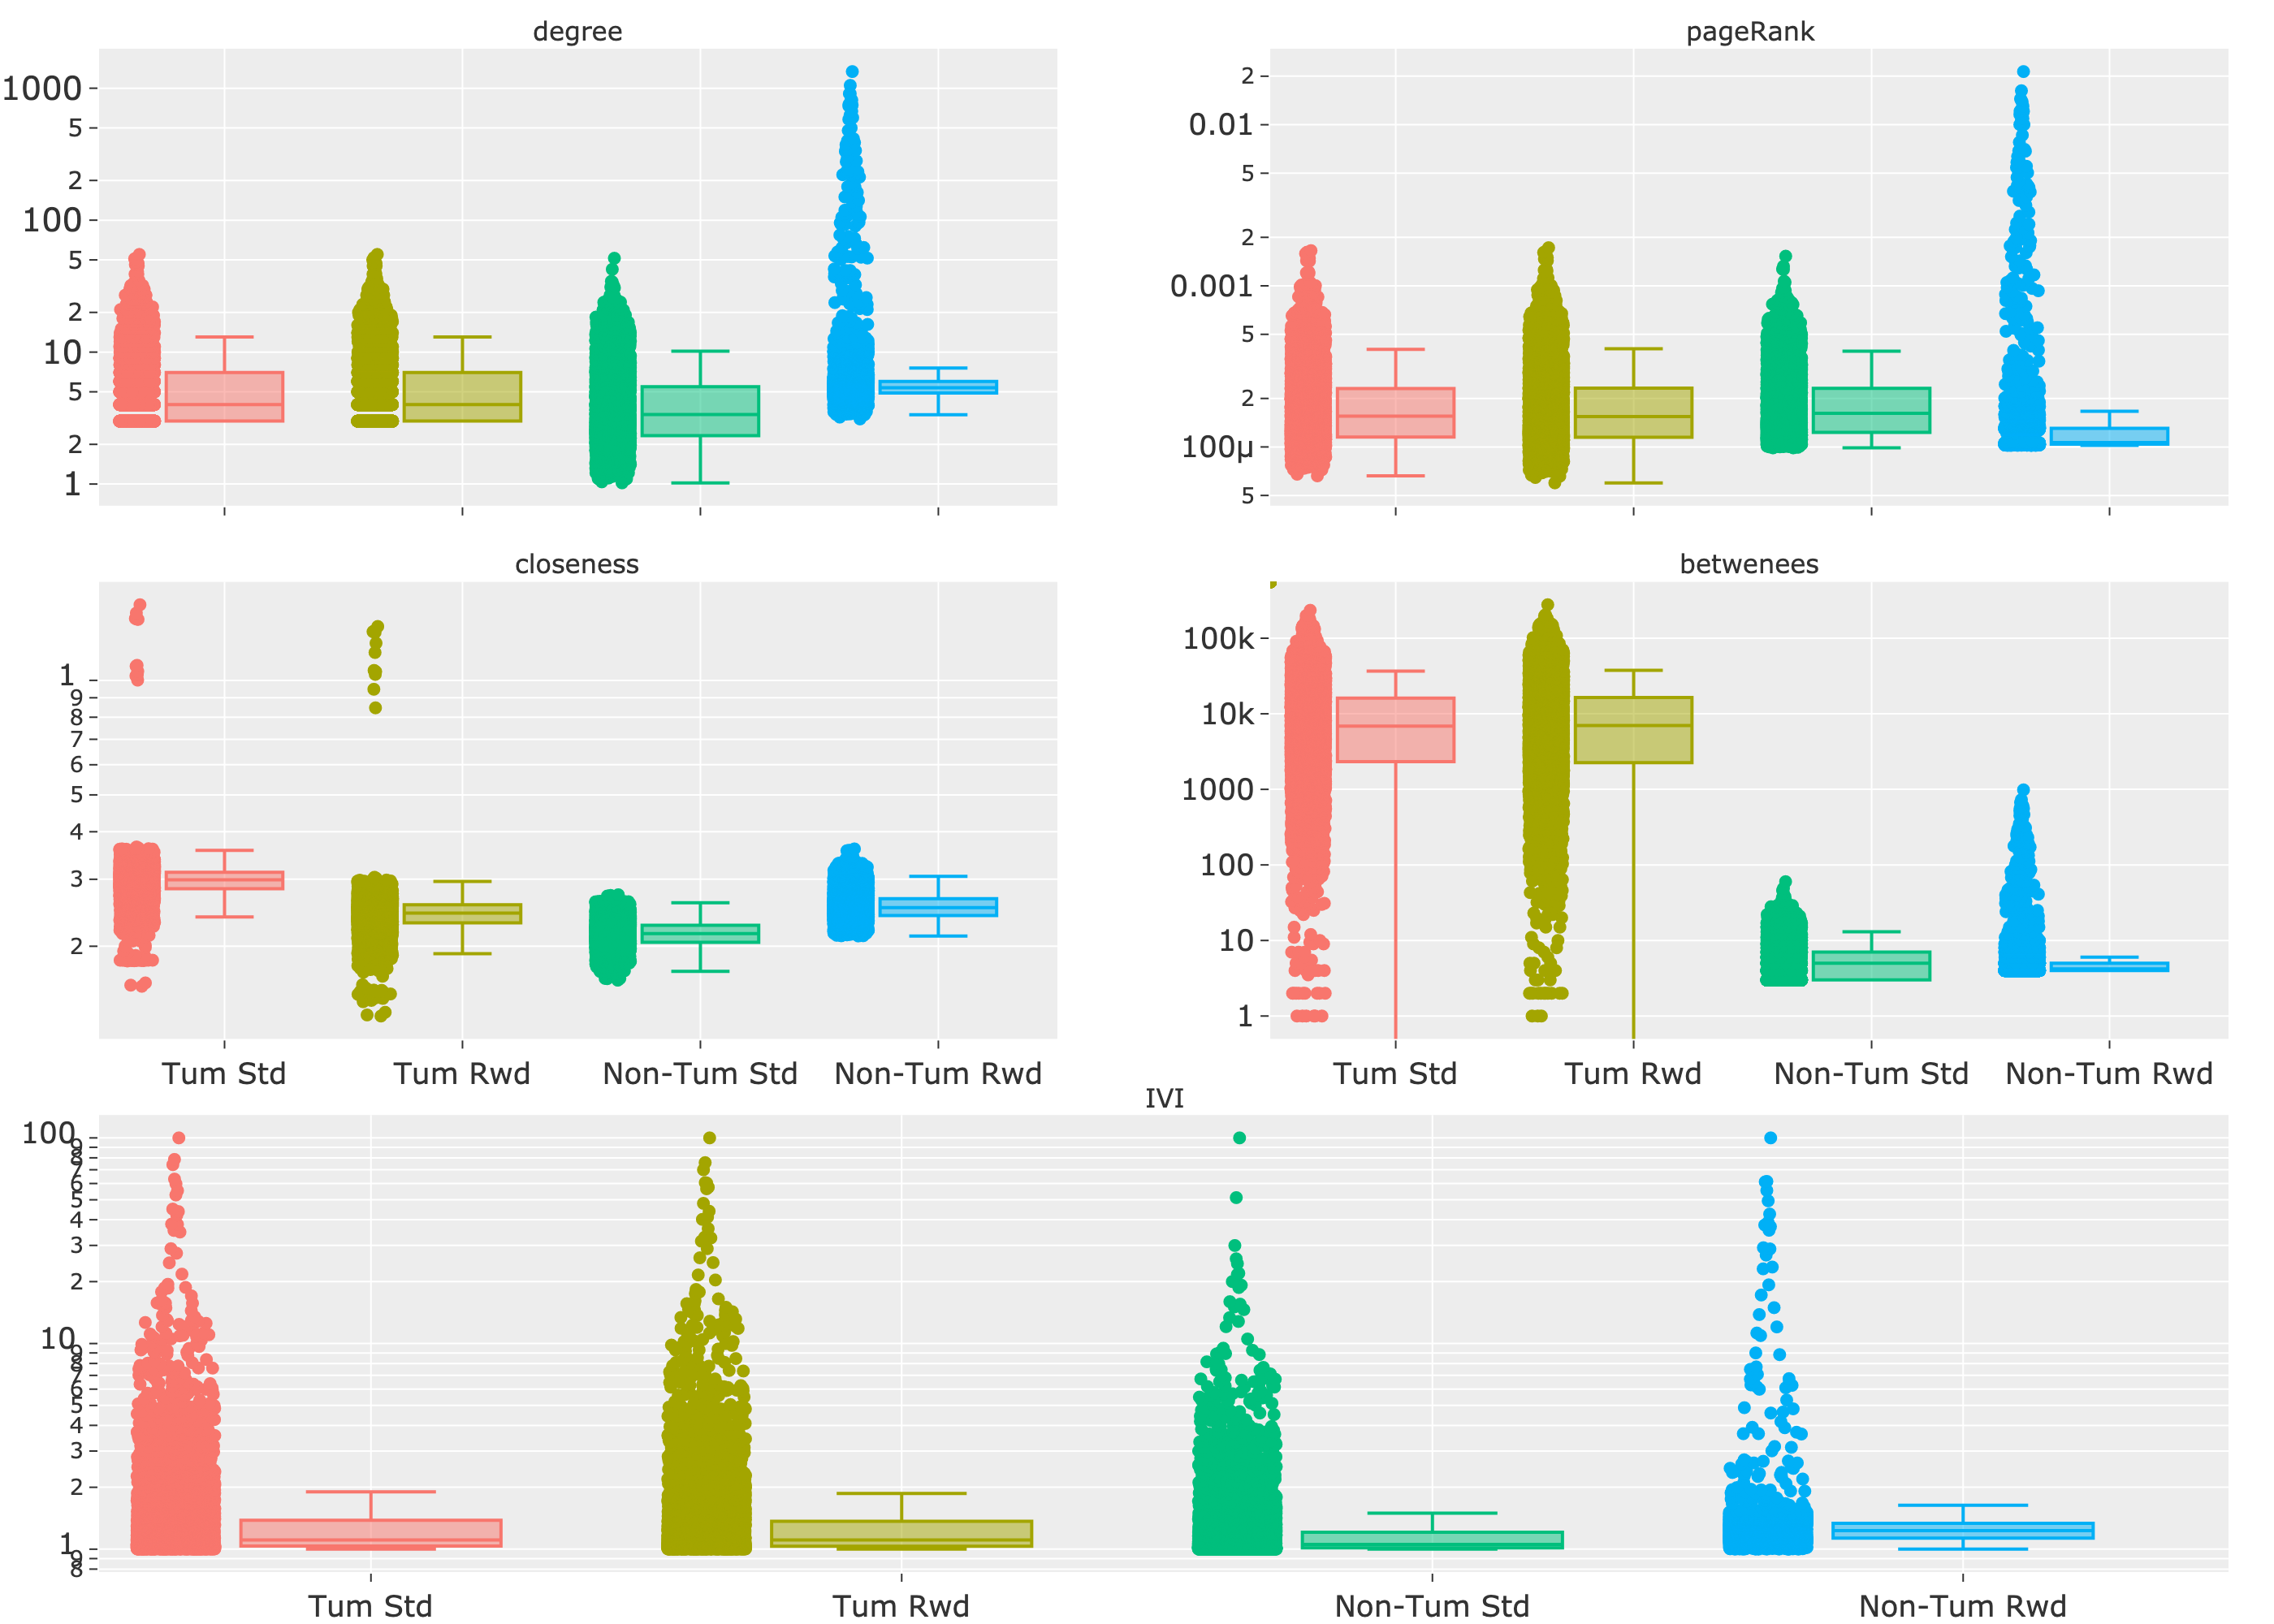
\includegraphics[width=1.0\textwidth,height=0.7\textheight,keepaspectratio]{Sections/Network_II/validation/network_comparison.png}
    \caption{Network metrics for the Tumour and non-tumour networks with no modifier and reward modifier. The y-axis represent the log10 of the metric. }
    \label{fig:N_II:net_metrics_comp}
\end{figure}

\subsubsection{Reward 1 vs Reward 2}

A sigmoid function is used as a reward modifier for the revised network pipeline presented in this chapter. The differences in how the weight are changed by the two functions are shown in \textbf{The two modifier functions}. 

The effect of the two modifiers can be seen in the networks \ref{}, the standard graphs are used as a control both the non-tumour and tumour datasets.


% Standard vs Reward
\subsubsection{Studying the sigmoid reward modifier}

% introduce the kaltz centrality
In the previous sections the network differences between the Standard and modified networks was studied through the bar plots. The comparisons involved three networks as 3 histograms on a single plot resulted on a cluttered figures. In this section, only the Standard and the Reward with sigmoid function are compared over the five usual clustering metrics utilised in this PhD project as well as the Katz Centrality metrics. The latter is a centrality metric available in the Graph-tool package\footnote{The Katz Centrality metric was available only in the Graph-tool package and not in the iGraph the package used by PGCNA to generated the graph.} which considers both the neighbours of a node as well as their connection over the network. Higher values means that the nodes is important both locally and globally in the network, while lower values are associated with less important roles. 

% Analyse the metrics
The six metric are shown in \cref{fig:N_II:net_metric_sig_std} where the x-axes represents the graph metric while the y-axes the log10 count, the orange is associated with the Reward and blue with the Standard network. Across all six plots there is a striking difference between the Standard and the Reward modifier,  in the latter graph the nodes' attributes are more spread compared to the unmodified network. This means that the nodes in the Standard graph have a relative similar importance, closeness into the network compared to the Reward which has a few number of genes that are highly connected, central to the network.
The distributions of the closeness metric suggests that the nodes in the modified graph are closer together compared to the un-modified one. All in all, the metrics suggests that the modifier have a large impact on to the network.


% Talk about the stats and the difference between the stats
\begin{figure}[H]    
    \centering
    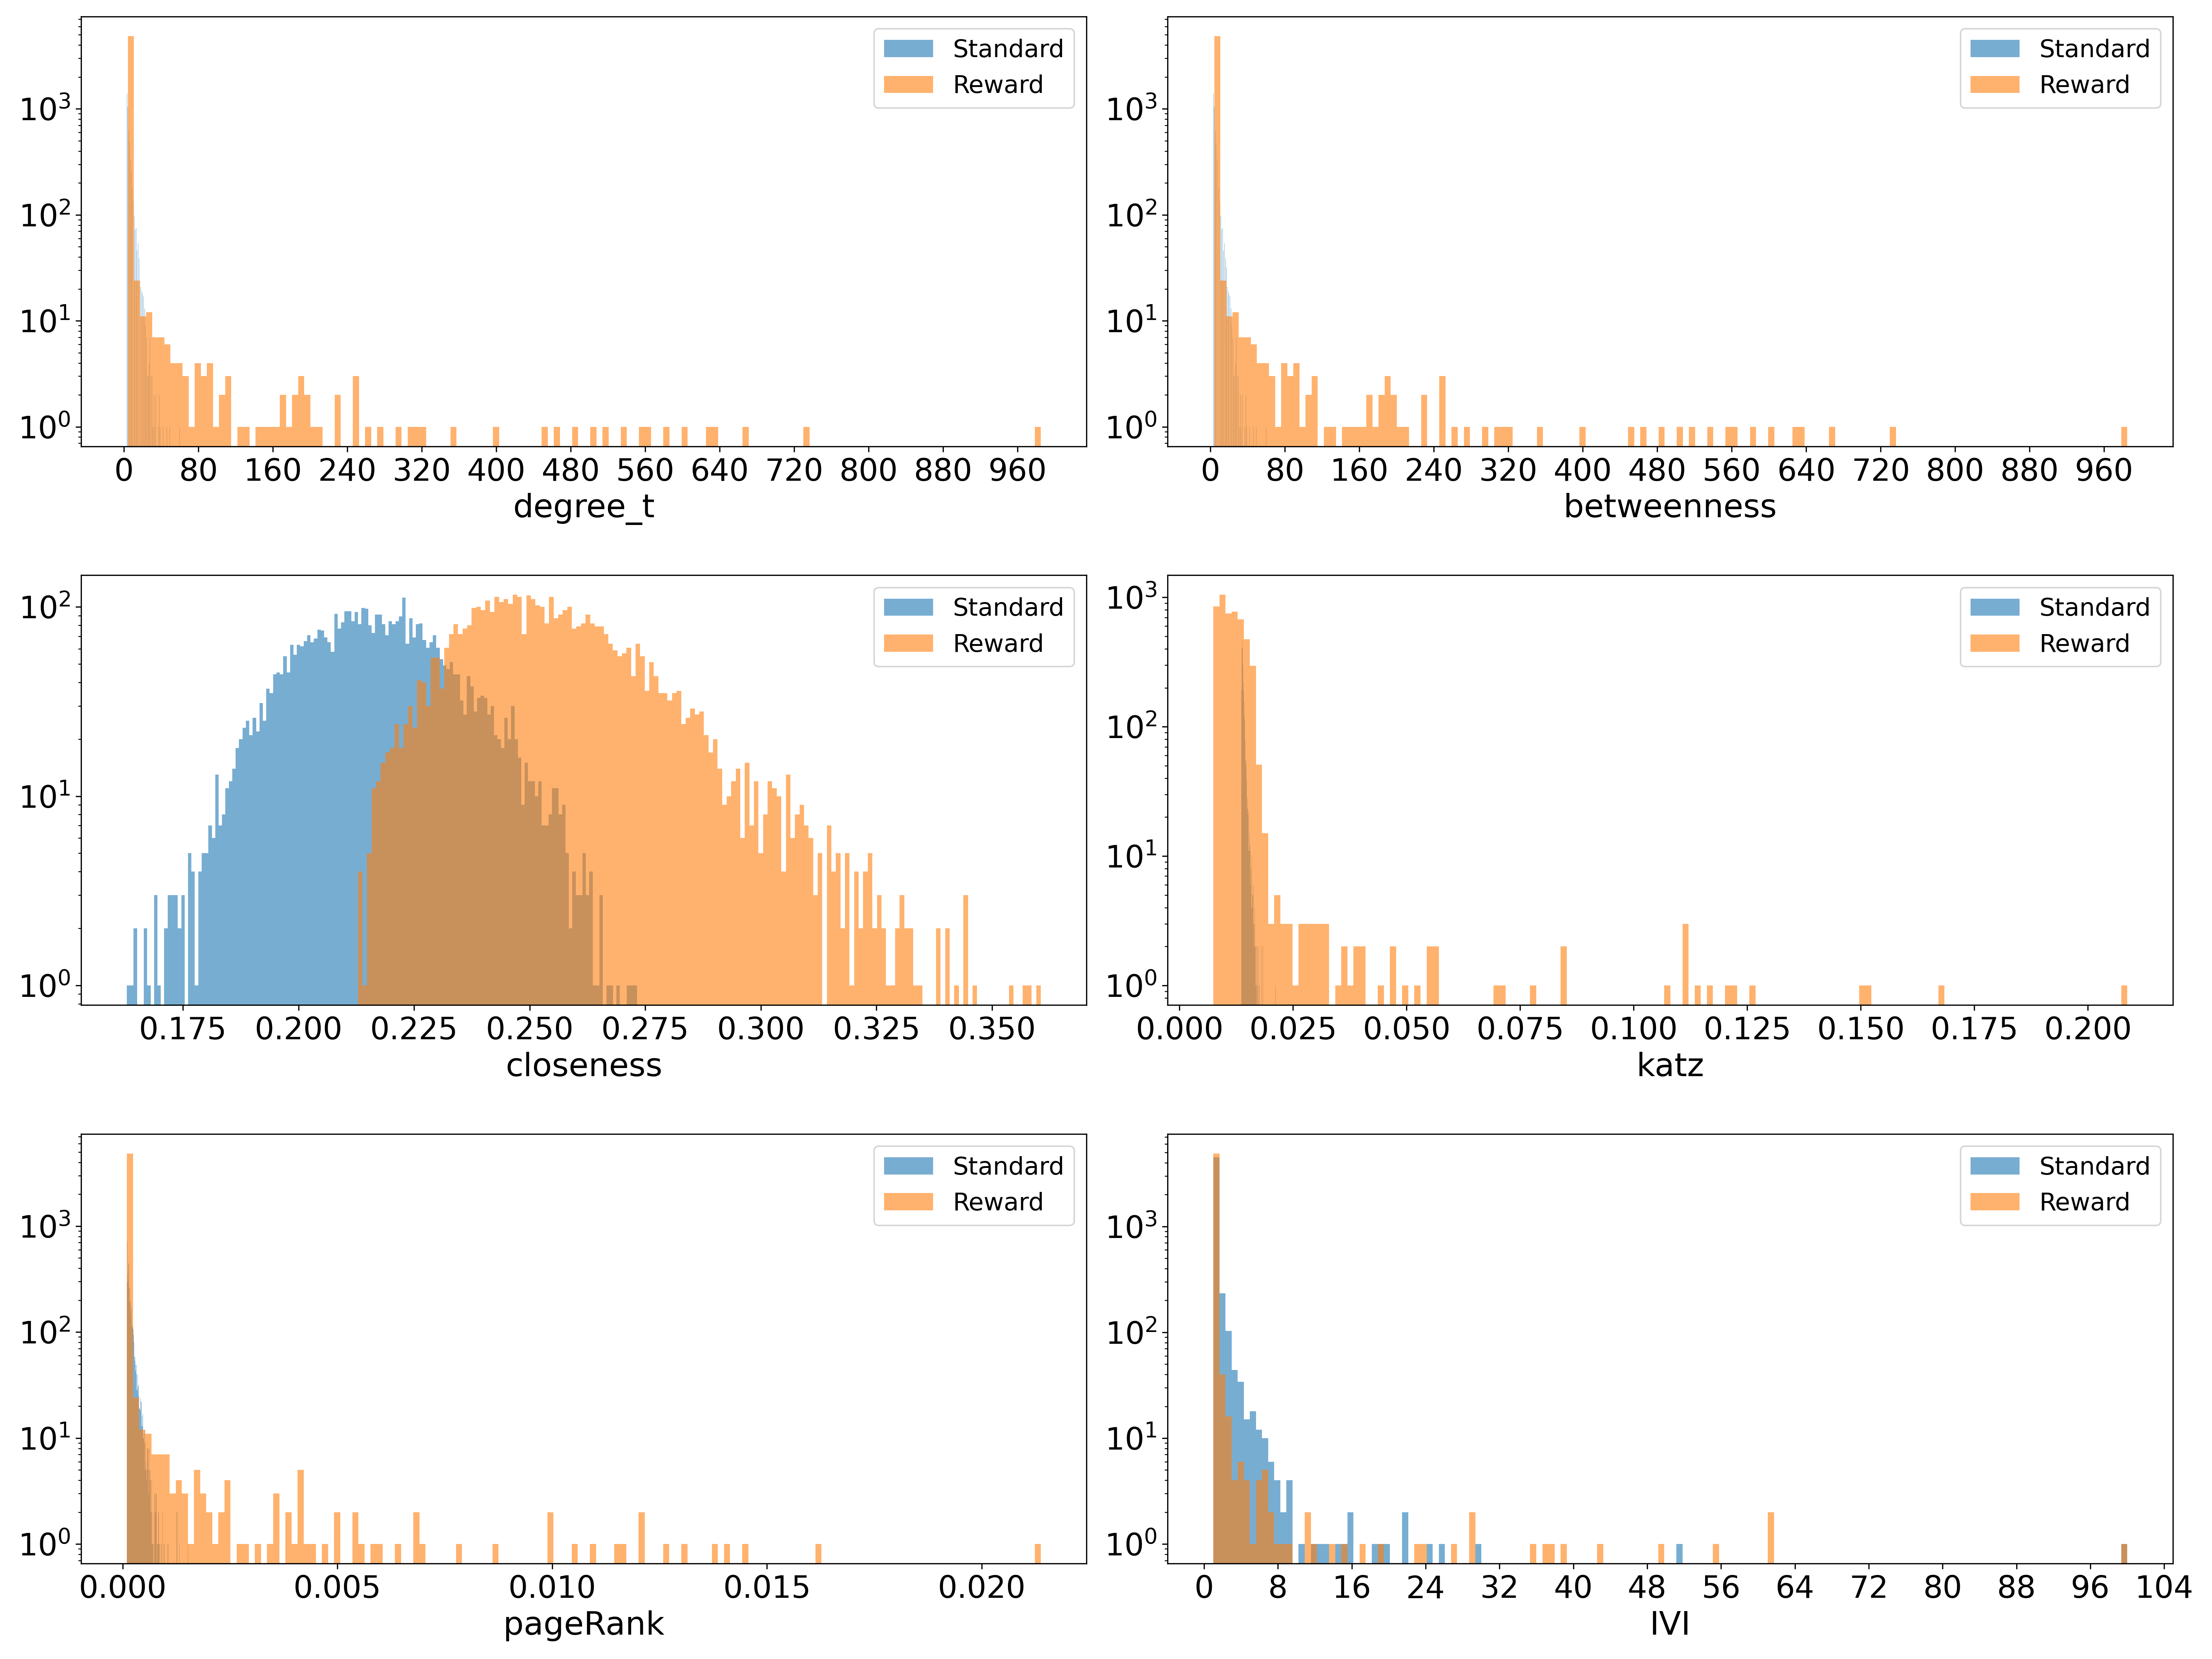
\includegraphics[width=1.0\textwidth,height=1.0\textheight,keepaspectratio]{Sections/Network_II/validation/net_metrics_Standard_Reward.png}
    \caption{Network metrics for the Standard and Sigmoid reward function. The y-axis represent the log10 of the count. }
    \label{fig:N_II:net_metric_sig_std}
\end{figure}



% Sigmoid function
% th

% Comparison between the weight modifiers

% SBM vs hSBM
\subsubsection{SBM vs hSBM}

% Community sizes
% Genes extracted


% iMev
\subsubsection{iMev - integrative MEV}

% Talk about how iMEV integrates the two gene expression datasets


How can we measure this change across the different networks.

\par\noindent\rule{\textwidth}{0.4pt}


This section will cover the usual plots used to analyse the networks.
\begin{todolist}
    \item[\done] Leiden Rank compared to the modifiers
    \item[\done] Sankey plot with stratification with other methods: VU+in-situ + TCGA and consensus
    \item[\done] Community enrichment patterns
    \item [\done] Survival plots.
    \item Survival tables with different checkpoints.
    \item Show the genes that are not found in community 5. Exhibiting the need for remapping of all the healthy datasets.
    \item Gene stats 
    \begin{todolist}
        \item How many genes are shared between the tumour and healthy? All healthy and all tumour? Selected healthy and all tumour / selected most varied?
        \item How many of the healthy genes are mutated?
    \end{todolist}
\end{todolist}
